\subsection{Entre Dos Tierras}
\label{subsec:entre-dos-tierras}

El mayor problema al que nos hemos enfrentado en este proyecto es la gestión de las tierras en las señales de audio. Inicialmente diseñamos el circuito para que las señales de audio se conectaran entre la entrada de audio y la tierra virtual del circuito analógico, pensando que las señales serían compatibles con la entrada del ADC al estar alimentadas con los mismos niveles de tensión que los que las generan.

Sin embargo, descubrimos posteriormente que los circuitos compartían la tierra de audio de la entrada directamente con la salida, por lo que se realizaba un cortocircuito directo entre la tierra de la alimentación (o alimentación negativa visto desde el amplificador de audio) y la tierra virtual, por lo que se cortocircuitaban 3.5 V. 

Esto era claro en el lado del MP3 ya que el cortocircuito era a través de un camino de baja impedancia y provocaba que se activara la protección, desactivando la salida de audio. Sin embargo, debido a la circuitería interna o a las conexiones de la radio, había una pequeña pero no mínima impedancia que provocaba un consumo muy elevado de corriente pero que no llegaba al amperio, por lo que la protección no se disparaba. Esto es muy peligroso ya que es una potencia que se está disipando en el interior del chip y probablemente provoque daños si se mantiene el circuito en dicha condición.

Para solucionar este problema, decidimos construir unos cables de sonido en los cuales solo se conecte el terminal que lleva la señal, deshaciendo la conexión que realizan los sensores internamente.

Con estos ajustes la radio funcionaba bien, sin demasiado problema (excepto el ruido del que hablaremos a continuación). Sin embargo, el MP3 presenta otro problema. Contraintuitivamente, a pesar de estar alimentado con una tensión unipolar, el circuito del MP3 consigue generar una tensión bipolar simétrica con la señal de audio, señal completamente incompatible con nuestro sistema de muestreo con un ADC de la placa.

Para mediar este problema, hemos montado otro circuito analógico accesorio que mediante un divisor de tensión simétrico y un condensador de desacoplo consigue añadir una componente continua de 1.65 V a la tensión simétrica de entrada, haciendola completamente compatible con el sistema. Se añade una resistencia de \textit{Pull-down} en la entrada para evitar picos de tensión en el encendido del sistema. Los valores de las resistencias pueden ser cualesquiera valores grandes siempre que sean iguales y el condensador interesa elegirlo lo más grande posible. El circuito está recogido en la \autoref{fig:2-6-sumador}. 

\begin{figure}[h]
    \centering
    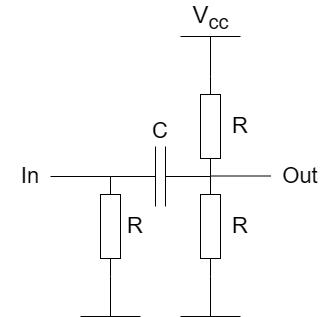
\includegraphics[width=0.5\textwidth]{images/2/2-6/sumadorEsquematico.png}
    \caption{Esquemático del circuito sumador}
    \label{fig:2-6-sumador}
\end{figure}

Se ha montado el circuito sobre una placa de baquelita, como se puede ver en la imagen de la TODO.\ 

% TODO: Imagen de la chapuza

Hemos elegido un valor de $100\ k\Omega$ para las resistencias y aproximadamente $1\ \mu F$ para el condensador, lo cual nos ofrece buenos resultados. Sin embargo, primero realizamos las pruebas con un condensador cerámico y no conseguimos que la tensión se estabilizara, por lo que se desplazaba el valor lentamente hacia uno de los raíles de alimentación. La solución que encontramos fue sustituirlo por un condensador de tántalo, que si bien tiene un tamaño físico considerablemente superior, consigue mantener de manera muy estable la tensión del circuito.

Este circuito funciona correctamente pero tiene la desventaja de decrementar ligeramente la tensión de entrada, provocando una caída en la relación señal-ruido del sistema.

Una vez solucionado el problema de las masas, aparece un ruido muy elevado en forma de zumbido y ruido blanco, por lo que el audio es de bastante baja relacion calidad ruido. Esto es principalmente debido a la longitud de los conductores por lo que va la señal, la cantidad de circuitos que atraviesa, etcétera. 

Además, la desconexión de las masas de los cables de audio provoca que el camino de retorno de las señales tenga que atravesar el resto del circuito y se deja de tratar la señal como un par diferencial, por lo que se pierde bastante calidad debido a la diferencia de tensión en las masas y algún posible bucle de masa al que se le acople algún ruido.

Por todo ello, si se quiere disfrutar de la máxima calidad de audio que puede ofrecer nuestro circuito, se debe desconectar la masa de la placa de la del circuito de amplificación de audio. El principal inconveniente de ello es que se deja de poder gestionar el multiplexor y la habilitación a través de los GPIO y no se puede realizar el procesado digital de señales.

Si se conectan los pines de selección y habilitación a los raíles de alimentación para seleccionar la configuración y se conecta un jumper entre los pines de ADC y DAC, se tiene una buenísima calidad de sonido, tanto en el altavoz como en los cascos. Se puede igualmente controlar la radio y el MP3 mediante las interfaces ya que eso no depende de la masa del circuito.

La mejor solución a este problema sería la realización de un circuito con alimentación simétrica verdadera. Esto se podría conseguir mediante dos baterías en serie (aunque sería un desperdicio ya que una solo se utilizaría para la parte negativa de la señal y no alimentaría la placa) o mediante la generación de una tensión negativa con un convertidor, por ejemplo, de tipo reductor-elevador con topología inversora. Igualmente se tendría que tener en cuenta la naturaleza bipolar de la señal del MP3 y se debería incluir el circuito de \textit{offset} a la placa o utilizar un cambiador de nivel analógico.